\documentclass[presentation,aspectratio=43, 10pt]{beamer}
\usepackage{pifont}
\newcommand{\cmark}{\ding{51}}
\newcommand{\xmark}{\ding{55}}

\titlegraphic{\hfill
\includegraphics[height=1.25cm]{durham-logo}}
\usepackage{appendixnumberbeamer}
\usepackage{amsmath}
\usepackage{amssymb}
\usepackage{mathtools}
\usepackage{hyperref}
\usepackage{xspace}
\newcommand{\arxivlink}[2]{{\texttt{arXiv:\,\href{https://arxiv.org/abs/#1}{#1\,[#2]}}}}

\newcommand{\honev}{\ensuremath{{H}^1(\Omega; \mathbb{R}^d)}\xspace}
\newcommand{\ltwov}{\ensuremath{{L}^2(\Omega; \mathbb{R}^d)}\xspace}
\newcommand{\ltwo}{\ensuremath{{L}^2(\Omega)}\xspace}
\newcommand{\inner}[1]{\left\langle #1 \right \rangle}


\usepackage{minted}
\usepackage[url=false,
doi=true,
isbn=false,
style=authoryear,
maxnames=5,
giveninits=true,
uniquename=init,
backend=biber]{biblatex}
\renewcommand{\bibfont}{\fontsize{7}{7}\selectfont}
\addbibresource{references.bib}

\setlength{\bibitemsep}{1ex}
\setlength{\fboxsep}{1pt}

\renewbibmacro{in:}{}
\DeclareFieldFormat[article]{volume}{\textbf{#1}}
\DeclareFieldFormat{doi}{%
  doi\addcolon%
  {\scriptsize\ifhyperref{\href{http://dx.doi.org/#1}{\nolinkurl{#1}}}
    {\nolinkurl{#1}}}}
\AtEveryBibitem{%
\clearfield{pages}%
\clearfield{issue}%
\clearfield{number}%
}

\DeclareMathOperator{\grad}{grad}
\let\div\relax
\DeclareMathOperator{\div}{div}
\DeclareMathOperator{\curl}{curl}
\DeclareMathOperator{\range}{range}
\usetheme{metropolis}
\setbeamertemplate{title graphic}{
  \vbox to 0pt {
    \vspace*{1em}
    \inserttitlegraphic%
  }%
  \nointerlineskip%
}
\metroset{background=light,progressbar=frametitle,numbering=counter,block=fill}

% https://www.dur.ac.uk/marketingandcommunications/marketing/branding/colourpalette/
% Most of these are indistinguishable to those suffering colour blindness
\definecolor{purple}{HTML}{7e317b}
\definecolor{lightpurple}{HTML}{D8ACE0}
\definecolor{blue}{HTML}{006388}
\definecolor{red}{HTML}{AA2B4A}
\definecolor{green}{HTML}{9FA161}
\definecolor{yellow}{HTML}{E8E391}
\definecolor{pink}{HTML}{C43B8E}
\definecolor{lightblue}{HTML}{C4E5FA}

\setbeamercolor{normal text}{
  fg=black,
  bg=white
}
\setbeamercolor{alerted text}{
  fg=red
}
\setbeamercolor{example text}{
  fg=blue
}

\setbeamercolor{palette primary}{%
  use=normal text,
  fg=normal text.bg,
  bg=purple,
}

\usetheme{metropolis}

\author{Lawrence Mitchell\inst{1,*} \\
  \and {\scriptsize
    P.~E.~Farrell (Oxford)
    \and
    R.~C.~Kirby (Baylor)
    \and
    M.~G.~Knepley (Buffalo)
    \and
    F.~Wechsung (Oxford)}}
\institute{
  \inst{1}Department of Computer Science, Durham University\\
  \inst{*}\texttt{lawrence.mitchell@durham.ac.uk}}

\title{Flexible computational abstractions for complex
  preconditioners}

\usepackage{tikz}
\usetikzlibrary{trees,calc,positioning}
\usetikzlibrary{shapes, shapes.geometric}
\usetikzlibrary{arrows,chains,positioning,fit,backgrounds,calc,shapes,
  shadows,scopes,decorations.markings,plotmarks}

\newcommand*{\tettextsize}{\footnotesize}
\tikzstyle{line} = [draw, -, thick]
\tikzstyle{nodraw} = [draw, fill, circle, minimum width=0pt, inner sep=0pt]
\tikzstyle{sieve} = [line, circle, font=\tettextsize, inner sep=0pt,
  minimum size=12pt]

\tikzstyle{cell} = [sieve, fill=blue!60]
\tikzstyle{facet} = [sieve, fill=green!35]
\tikzstyle{edge} = [sieve, fill=red!35]
\tikzstyle{vertex} = [sieve, fill=blue!35]

% https://tex.stackexchange.com/questions/27171/padded-boundary-of-convex-hull
\newcommand{\convexpath}[2]{
  [
  create hullcoords/.code={
    \global\edef\namelist{#1}
    \foreach [count=\counter] \nodename in \namelist {
      \global\edef\numberofnodes{\counter}
      \coordinate (hullcoord\counter) at (\nodename);
    }
    \coordinate (hullcoord0) at (hullcoord\numberofnodes);
    \pgfmathtruncatemacro\lastnumber{\numberofnodes+1}
    \coordinate (hullcoord\lastnumber) at (hullcoord1);
  },
  create hullcoords
  ]
  ($(hullcoord1)!#2!-90:(hullcoord0)$)
  \foreach [
  evaluate=\currentnode as \previousnode using \currentnode-1,
  evaluate=\currentnode as \nextnode using \currentnode+1
  ] \currentnode in {1,...,\numberofnodes} {
    let \p1 = ($(hullcoord\currentnode) - (hullcoord\previousnode)$),
    \n1 = {atan2(\y1,\x1) + 90},
    \p2 = ($(hullcoord\nextnode) - (hullcoord\currentnode)$),
    \n2 = {atan2(\y2,\x2) + 90},
    \n{delta} = {Mod(\n2-\n1,360) - 360}
    in
    {arc [start angle=\n1, delta angle=\n{delta}, radius=#2]}
    -- ($(hullcoord\nextnode)!#2!-90:(hullcoord\currentnode)$)
  }
}

\graphicspath{{./\jobname.figures/}{../pictures/}}

\begin{document}

\maketitle

% \begin{abstract}
%   Small block overlapping, and non-overlapping, Schwarz methods are
%   theoretically highly attractive as multilevel smoothers for a wide
%   variety of problems that are not amenable to point relaxation
%   methods.  Examples include monolithic Vanka smoothers for Stokes,
%   overlapping vertex-patch decompositions for $H(\text{div})$ and
%   $H(\text{curl})$ problems, along with nearly incompressible
%   elasticity, and augmented Lagrangian schemes.

%   While it is possible to manually program these different schemes,
%   their use in general purpose libraries has been held back by a lack
%   of generic, composable interfaces. We present a new approach to the
%   specification and development such additive Schwarz methods in PETSc
%   that cleanly separates the topological space decomposition from the
%   discretisation and assembly of the equations. Our preconditioner is
%   flexible enough to support overlapping and non-overlapping additive
%   Schwarz methods, and can be used to formulate line, and plane
%   smoothers, Vanka iterations, amongst others. I will illustrate these
%   new features with some examples utilising the Firedrake finite
%   element library, in particular how the design of an approriate
%   computational interface enables these schemes to be used as building
%   blocks inside block preconditioners.

%   This is joint work with Patrick Farrell and Florian Wechsung
%   (Oxford), Rob Kirby (Baylor), and Matt Knepley (Buffalo).
% \end{abstract}

\begin{frame}[t]
  \frametitle{Setting}

  \begin{overlayarea}{\textwidth}{\textheight}
    \begin{onlyenv}<1>
      \begin{columns}
        \begin{column}{0.8\textwidth}
          \begin{quote}
            Firedrake \url{www.firedrakeproject.org} {\normalfont
              [\ldots]} is an automated system for the solution of
            partial differential equations using the finite element
            method.
          \end{quote}
        \end{column}
        \begin{column}{0.2\textwidth}
          
\includegraphics[width=0.8\textwidth]{firedrake-small}
        \end{column}
      \end{columns}
      \begin{itemize}
      \item Written in Python.
      \item Finite element problems specified with \emph{embedded}
        domain specific language, UFL \parencite{Alnaes:2014} from the
        FEniCS project.
      \item \emph{Runtime} compilation to optimised, low-level (C)
        code.
      \item PETSc for meshes and (algebraic) solvers.
      \end{itemize}

      \begin{flushright}
        {\scriptsize \textcite{Rathgeber:2016} \arxivlink{1501.01809}{cs.MS}}
      \end{flushright}
    \end{onlyenv}
    \begin{onlyenv}<2>
      \begin{block}{Particular strengths}
        \begin{itemize}
        \item Geophysical fluid dynamics (one structured dimension)

        \item Transparently parallel
        \item All\textsuperscript{(*)} the finite elements
        \end{itemize}

        \textsuperscript{(*)} Not actually all of them
      \end{block}
      \begin{block}{User groups}
        \begin{itemize}
        \item Imperial, Oxford, Bath, Leeds, Durham, Kiel, Rice,
          Houston, Exeter, Buffalo, Waterloo, Minnesota, Baylor, Texas
          A\&M, \dots
        \item Annual user \& developer meeting this year had 45
          attendees.
        \item Next meeting (2019) probably in Durham in September.
        \end{itemize}
      \end{block}
    \end{onlyenv}
  \end{overlayarea}
\end{frame}

\begin{frame}[fragile,t]
  \frametitle{UFL makes it easy to write complex PDEs}
  \begin{onlyenv}<1>
    \begin{columns}[T]
      \begin{column}{0.47\framewidth}
        \small
        \begin{block}{Rayleigh-B\'enard convection}
          \begin{equation*}
            \begin{split}
              -\Delta u + u\cdot\nabla u + \nabla p +
              \frac{\text{Ra}}{\text{Pr}} \hat{g}T &= 0 \\
              \nabla \cdot u &= 0 \\
              - \frac{1}{\text{Pr}} \Delta T + u\cdot \nabla T &= 0
            \end{split}
          \end{equation*}
          Newton
          \begin{equation*}
            \begin{bmatrix}
              F   & B^T & M_1 \\
              C   & 0   & 0   \\
              M_2 & 0 & K
            \end{bmatrix}
            \begin{bmatrix}
              \delta u \\
              \delta p \\
              \delta T
            \end{bmatrix} =
            \begin{bmatrix}
              f_1 \\
              f_2 \\
              f_3
            \end{bmatrix}
          \end{equation*}
        \end{block}
      \end{column}
      \begin{column}{0.52\framewidth}
\begin{minted}[fontsize=\tiny]{python}
from firedrake import *
mesh = Mesh(...)
V = VectorFunctionSpace(mesh, "CG", 2)
W = FunctionSpace(mesh, "CG", 1)
Q = FunctionSpace(mesh, "CG", 1)
Z = V * W * Q
Ra = Constant(200)
Pr = Constant(6.18)
upT = Function(Z)
u, p, T = split(upT)
v, q, S = TestFunctions(Z)
bcs = [...] # no-flow + temp gradient
nullspace = MixedVectorSpaceBasis(
   Z, [Z.sub(0), VectorSpaceBasis(constant=True),
       Z.sub(2)])
F = (inner(grad(u), grad(v))
     + inner(dot(grad(u), u), v)
     - inner(p, div(v))
     + (Ra/Pr)*inner(T*g, v)
     + inner(div(u), q)
     + inner(dot(grad(T), u), S)
     + (1/Pr) * inner(grad(T), grad(S)))*dx

solve(F == 0, upT, bcs=bcs, nullspace=nullspace)
\end{minted}
      \end{column}
    \end{columns}
  \end{onlyenv}
  \begin{onlyenv}<2>
    \begin{columns}[T]
      \begin{column}{0.47\textwidth}
        \begin{block}{Ohta--Kawasaki}
          \small
          \begin{align*}
            u_t - \Delta w + \sigma(u - m) &= 0\\
            w + \epsilon^2 \Delta u - u(u^2 - 1) &= 0
          \end{align*}
          Implicit timestepping + Newton
          \begin{equation*}
            \begin{bmatrix}
              (1 + \Delta t \theta \sigma)M  & \Delta t\theta K \\
              -\epsilon^2 K - M_E & M
            \end{bmatrix}
            \begin{bmatrix}
              \delta u \\
              \delta w
            \end{bmatrix} =
            \begin{bmatrix}
              f_1 \\
              f_2
            \end{bmatrix}
          \end{equation*}
        \end{block}
      \end{column}
      \begin{column}{0.52\textwidth}
\begin{minted}[fontsize=\tiny,escapeinside=||]{python}
from firedrake import *
mesh = Mesh(...)
V = FunctionSpace(mesh, "CG", 1)
Z = V*V
|$\epsilon$| = Constant(0.02)
|$\sigma$| = Constant(100)
dt = Constant(eps**2)
|$\theta$| = Constant(0.5)
v, q = TestFunctions(Z)
z = Function(Z)
z0 = Function(Z)
u, w = split(z)
u0, w0 = split(z0)
u|$_\theta$| = (1 - |$\theta$|)*u0 + |$\theta$|*u
w|$_\theta$| = (1 - |$\theta$|)*w0 + |$\theta$|*w
dfdu = u**3 - u
F = ((u - u0)*v
     + dt*dot(grad(w|$_\theta$|), grad(v))
     + dt*|$\sigma$|*(u|$_\theta$| - m)*v
     + w*q - dfdu*q
     - |$\epsilon$|**2*dot(grad(u), grad(q)))*dx
while t < ...:
    z0.assign(z)
    solve(F == 0, z)
\end{minted}
      \end{column}
    \end{columns}
  \end{onlyenv}
\end{frame}


\begin{frame}[standout]
  What about the solvers?
\end{frame}

\begin{frame}[t]
  \frametitle{Some motivating problems: block preconditioners}

  \begin{onlyenv}<1>
    \begin{block}{Stokes equations}
      \begin{alignat*}{2}
        -\nabla^2 u + \nabla p &= f \quad && \text{ in } \Omega, \\
        \nabla \cdot u &= 0 \quad && \text{ in } \Omega, \\
      \end{alignat*}

      Discretising with inf-sup stable element pair results in:
      \begin{equation*}
        Jx := \begin{bmatrix}
          A & B^T \\
          B & 0
        \end{bmatrix}
        \begin{bmatrix}
          u \\ p
        \end{bmatrix}
        =
        \begin{bmatrix}
          b \\ 0
        \end{bmatrix}.
      \end{equation*}
    \end{block}
  \end{onlyenv}
  \begin{onlyenv}<2>
    \begin{block}{\dots and a preconditioner}
      Use a diagonal Schur complement factorisation
      \parencite{Silvester:1994}
      \begin{equation*}
        \tilde{J}^{-1} =
        \begin{bmatrix}
          \tilde{A}^{-1}  & 0 \\
          0 & \tilde{S}^{-1} \\
        \end{bmatrix}
      \end{equation*}

      With multigrid for $\tilde{A}^{-1}$, and
      $\tilde{S}^{-1} = -Q^{-1}$ ($Q$ the pressure mass matrix).
    \end{block}
  \end{onlyenv}
  \begin{onlyenv}<3>
    \begin{block}{Stationary Rayleigh-B\'enard convection}
      \begin{equation*}
        \begin{split}
          -\Delta u + u\cdot\nabla u + \nabla p +
          \frac{\text{Ra}}{\text{Pr}} \hat{g}T &= 0 \\
          \nabla \cdot u &= 0 \\
          - \frac{1}{\text{Pr}} \Delta T + u\cdot \nabla T &= 0
        \end{split}
      \end{equation*}
      Newton linearisation
      \begin{equation*}
        \begin{bmatrix}
          F   & B^T & M_1 \\
          C   & 0   & 0   \\
          M_2 & 0 & K
        \end{bmatrix}
        \begin{bmatrix}
          \delta u \\
          \delta p \\
          \delta T
        \end{bmatrix} =
        \begin{bmatrix}
          f_1 \\
          f_2 \\
          f_3
        \end{bmatrix}
      \end{equation*}
    \end{block}
  \end{onlyenv}
  \begin{onlyenv}<4>
    \begin{block}{\dots and a preconditioner}
      {\small For each Newton step, invert the $3\times 3$ block
        system using the preconditioner of \textcite{Howle:2012}:
        \begin{equation*}
          \begin{bmatrix}
            \widetilde{\begin{bmatrix}
                F & B^T\\
                C & 0
              \end{bmatrix}}^{-1} & 0\\
            0 & I
          \end{bmatrix}
          \begin{bmatrix}
            I & 0 & -M_1\\
            0 & I & 0 \\
            0 & 0 & I
          \end{bmatrix}
          \begin{bmatrix}
            I & 0 & 0\\
            0 & I & 0\\
            0 & 0 & \tilde{K}^{-1}
          \end{bmatrix}
        \end{equation*}
        with
        \begin{equation*}
          \widetilde{\begin{bmatrix}
              F & B^T\\
              C & 0
            \end{bmatrix}}^{-1} = \begin{bmatrix}
            F & 0 \\
            0 & \tilde{S}^{-1}
          \end{bmatrix}
          \begin{bmatrix}
            I & 0\\
            -C & I
          \end{bmatrix}
          \begin{bmatrix}
            \tilde{F}^{-1} & 0 \\
            0 & I
          \end{bmatrix}
        \end{equation*}
        with $S = -C \tilde{F}^{-1} B^T$ the Schur complement, whose
        inverse is approximated with PCD:
        \begin{equation*}
          \tilde{S}^{-1} = \tilde{M}_p^{-1}(\mathbb{I} + F_p \tilde{L}_p^{-1})
        \end{equation*}
      }
    \end{block}
  \end{onlyenv}
  \begin{onlyenv}<5>
    \begin{block}{Ohta--Kawasaki equation: phase separation in
        polymers}
      \begin{equation*}
        \begin{split}
          u_t - \Delta w + \sigma(u - m) &= 0\\
          w + \epsilon^2 \Delta u - u(u^2 - 1) &= 0
        \end{split}
      \end{equation*}
      Newton linearisation
      \begin{equation*}
        \begin{bmatrix}
          (1 + \Delta t \theta \sigma)M  & \Delta t\theta K \\
          -\epsilon^2 K - M_E & M
        \end{bmatrix}
        \begin{bmatrix}
          \delta u \\
          \delta w
        \end{bmatrix} =
        \begin{bmatrix}
          f_1 \\
          f_2
        \end{bmatrix}
      \end{equation*}
    \end{block}
  \end{onlyenv}
  \begin{onlyenv}<6>
    \begin{block}{\dots and a preconditioner}
      For each Newton step, invert the $2\times 2$ block system using
      a preconditioner from \textcite{Farrell:2017}:
      \begin{equation*}
        \begin{bmatrix}
          \left[(1 + \Delta t \theta \sigma)M\right]^{-1}  & 0 \\
          0 & \widetilde{S}^{-1}
        \end{bmatrix}
        \begin{bmatrix}
          I & 0\\
          (\epsilon^2 K + M_E)\left[(1 + \Delta t \theta
              \sigma)M\right]^{-1} & I\\
        \end{bmatrix}.
      \end{equation*}
      Where the Schur complement is preconditioned by
      \begin{equation*}
        \tilde{S}^{-1} = \hat{S}^{-1}M\hat{S}^{-1}
      \end{equation*}
      with
      \begin{equation*}
        \hat{S} = M + \epsilon\sqrt{(\Delta t \theta)/(1+\Delta t \theta\sigma)} K.
      \end{equation*}
    \end{block}
  \end{onlyenv}
  \begin{onlyenv}<7>
    \begin{block}{Time dependent Stokes}
      Implicit time-stepping schemes lead to a saddle-point system
      \begin{equation*}
        \begin{bmatrix}
          I - \epsilon^2 \Delta & -\grad\\
          \div & 0
        \end{bmatrix}.
      \end{equation*}
      For which the ``canonical'' diagonal block preconditioner is
      \begin{equation*}
        \begin{bmatrix}
          (I - \epsilon^2 \Delta)^{-1} & 0\\
          0 & (-\Delta)^{-1} + \epsilon^2 I
        \end{bmatrix}.
      \end{equation*}
      \begin{flushright}
        \textcite{Mardal:2011} \hspace{4em}
      \end{flushright}
    \end{block}
  \end{onlyenv}
\end{frame}

\begin{frame}
  \frametitle{Unifying observation}
  \begin{block}{Auxiliary operators}
    Many schemes require access, \emph{in the preconditioner}, to
    matrix blocks that are not in the original operator.
  \end{block}
  \begin{example}
    \begin{itemize}
    \item PCD requires a pressure Laplacian, mass matrix, and
      convection
    \item Time dependent Stokes needs a pressure Laplacian, and mass
      matrix
    \end{itemize}
  \end{example}
  \begin{itemize}
  \item These operators are typically \emph{easy} for the
    discretisation library to build.
  \item How do we get them into the solver?
  \end{itemize}
\end{frame}

\begin{frame}
  \frametitle{Idea: ``\texttt{PCFIREDRAKE}''}
  \begin{itemize}
  \item Endow discretised operators with PDE-level information:
    \begin{itemize}
    \item what equation/function space?
    \item boundary conditions, etc\ldots
    \end{itemize}
  \item Enable use of PETSc's \texttt{fieldsplit} preconditioner for
    these operators
  \item[$\Rightarrow$] gets access to all the block factorisation
    schemes
  \end{itemize}

  \begin{block}{Extend PETSc with Firedrake-level (discretisation) preconditioners}
    \begin{itemize}
    \item[\cmark] PETSc provides \emph{algebraic} composition of solvers. \nocite{Brown:2012}

    \item[\cmark] Firedrake can provide auxiliary operators

    \item[\xmark?] Require model developer to write a preconditioner
    \end{itemize}
  \end{block}
  \begin{flushright}
    \textcite{Kirby:2018} \arxivlink{1706.01346}{cs.MS} \hspace{4em}
  \end{flushright}
\end{frame}

\begin{frame}[fragile]
  \frametitle{That sounds like hard work}

  \begin{itemize}
  \item Thanks to Python, and \texttt{petsc4py}, it's not as bad as
    it sounds.
  \item We just write a little Python class that implements the
    application of the preconditioner
  \item For auxiliary operators, Firedrake provides some extra
    sugar.
  \item PETSc manages all the splitting and nesting already. So this
    does the right thing \emph{inside} multigrid, etc\ldots
  \end{itemize}
  \begin{block}{That Stokes PC}
    \begin{equation*}
      \begin{bmatrix}
        \tilde{A}^{-1} & 0 \\
        0 & \tilde{Q}^{-1}
      \end{bmatrix}
      \begin{bmatrix}
        A & B^T \\
        B & 0
      \end{bmatrix}
    \end{equation*}
  \end{block}
\end{frame}

\begin{frame}[fragile]
  \frametitle{Example: Stokes again}
\begin{minted}[fontsize=\scriptsize]{python}
from firedrake import *                  # Params set up as
...                                      -ksp_type gmres
V = VectorFunctionSpace(mesh, "P", 2)    -pc_type fieldsplit
Q = FunctionSpace(mesh, "P", 1)          -pc_fieldsplit_type schur
W = V*Q                                  -pc_fieldsplit_schur_fact_type diag
v, q = TestFunctions(W)                  -fieldsplit_0_
                                            -ksp_type preonly
w = Function(W)                             -pc_type gamg
u, p = split(w)                          -fieldsplit_1_
F = (inner(grad(u), grad(v))*dx             -ksp_type chebyshev
    - p*div(v)*dx - div(u)*q*dx             -ksp_max_it 2
                                            -pc_type python
                                            # Callback to Firedrake
class MassMatrix(AuxiliaryOperatorPC):      -pc_python_type MassMatrix
    _prefix = "mass_"                       -mass_pc_type sor
    def form(self, pc, test, trial):
        a = -inner(test, trial)*dx
        return (a, None)

solve(F == 0, w, solver_parameters=params)
\end{minted}
\end{frame}

\begin{frame}[fragile]
  \frametitle{Example: Ohta--Kawasaki}
  \begin{block}{Schur complement approximation}
    \begin{equation*}
      \tilde{S}^{-1} = \hat{S}^{-1}M\hat{S}^{-1}
    \end{equation*}
    where
    \begin{equation*}
      \hat{S} = M + \epsilon\sqrt{(\Delta t \theta)/(1+\Delta t \theta\sigma)} K.
    \end{equation*}
  \end{block}
  \begin{columns}[T]
    \begin{column}{0.49\textwidth}
\begin{minted}[fontsize=\tiny,mathescape,escapeinside=||]{python}
class OKPC(PCBase):
    def setUp(self, pc):
        _, P = pc.getOperators()
        ctx = P.getPythonContext()
        # User information about $\Delta t$, $\theta$, etc...
        dt, |$\theta$|, |$\epsilon$|, |$\sigma$| = ctx.appctx["parameters"]
        V = ctx.a.arguments()[0].function_space()
        c = (dt * |$\theta$|)/(1 + dt * |$\theta$| * |$\sigma$|)
        w = TrialFunction(V)
        q = TestFunction(V)
        # $\hat{S} = \inner{q, w} + \epsilon\sqrt{c}\inner{\nabla q, \nabla w}$, $c = \frac{\Delta t \theta}{1 + \Delta t \theta \sigma}$
        op = assemble(inner(w, q)*dx + 
                      |$\epsilon$|*sqrt(c)*inner(grad(w), grad(q))*dx)
        self.ksp = KSP().create(comm=pc.comm)
        self.ksp.setOptionsPrefix(pc.getOptionsPrefix + "hats_")
        self.ksp.setOperators(op, op)
        self.ksp.setFromOptions()
        self.mass = assemble(w*q*dx)
\end{minted}
    \end{column}
    \begin{column}{0.49\textwidth}
\begin{minted}[fontsize=\tiny,escapeinside=||,mathescape=true]{python3}
    def apply(self, pc, x, y):
        t1, t2 = self.work
        # $t_1 \leftarrow \hat{S}^{-1}x$
        self.ksp.solve(x, t1)
        # $t_2 \leftarrow M t_1$
        self.mass.mult(t1, t2)
        # $y \leftarrow \hat{S}^{-1}t_2 = \hat{S}^{-1} M \hat{S}^{-1} x$
        self.ksp.solve(t2, y)
\end{minted}
    \end{column}
  \end{columns}
\end{frame}

\section{Solvers on the blocks}

\begin{frame}
  \frametitle{Now that I have a hammer\ldots}
  \ldots can I find some nails?

  \begin{itemize}
  \item This approach gets me auxiliary operators
  \item and \emph{algebraic} solvers for the blocks
  \item Many hard problems require multigrid 
  \item \dots with something other than point smoothers
  \end{itemize}
  \pause

  \begin{center}
    $\Rightarrow$ Overlapping Schwarz methods
  \end{center}
\end{frame}

\begin{frame}
  \frametitle{Some motivating problems: multigrid smoothers}
  \begin{onlyenv}<1>
    \begin{block}{Coupled multigrid for Stokes/Navier--Stokes}
      In the SCGS scheme four velocites and one pressure
      corresponding to one finite difference node are simultaneously
      updated by inverting a (small) matrix of equatioins.

      \begin{center}
        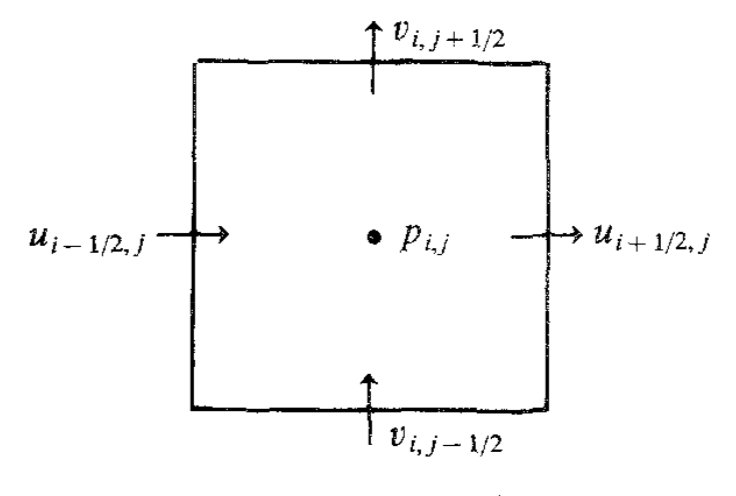
\includegraphics[height=3cm]{vanka}
      \end{center}
      \begin{flushright}
        \textcite{Vanka:1986} \hspace{4em}
      \end{flushright}
    \end{block}
  \end{onlyenv}
  \begin{onlyenv}<2>
    \begin{block}{$p$-independent preconditioners for elliptic problems}
      [Each subspace is generated from]
      $V_i^p = V^p \cap H^1_0(\Omega_i^{'})$ where $\Omega_i^{'}$ is the open square
      centered at the ith vertex
      \begin{center}
        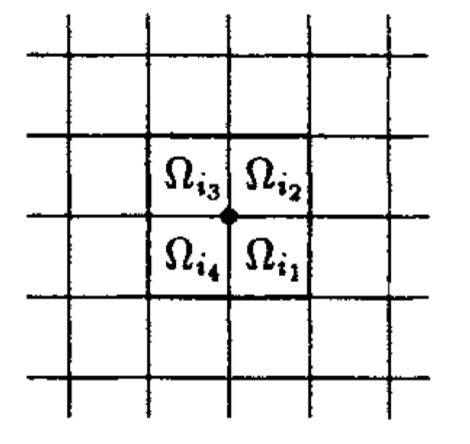
\includegraphics[width=3cm]{pavarino}
      \end{center}
      \begin{flushright}
        \textcite{Pavarino:1993} \hspace{4em}
      \end{flushright}
    \end{block}
  \end{onlyenv}

  \begin{onlyenv}<3>
    \begin{block}{Multigrid for nearly incompressible elasticity}
      The suggested smoother is block Jacobi smoother, which takes
      care of the kernel [...]. These kernel basis functions are
      captured by subspaces $V_{l,i}$ as shown
      \begin{center}
        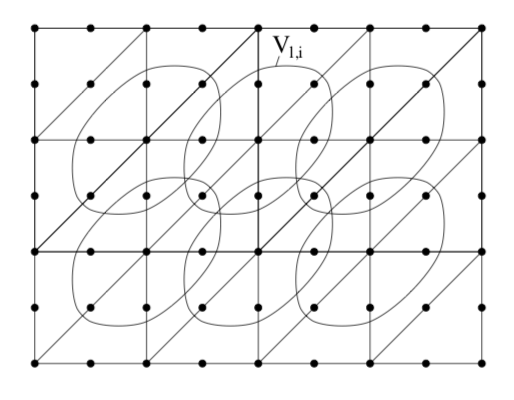
\includegraphics[height=3cm]{schoeberl}
      \end{center}
      \begin{flushright}
        \textcite{Schoeberl:1999} \hspace{4em}
      \end{flushright}
    \end{block}
  \end{onlyenv}

  \begin{onlyenv}<4>
    \begin{block}{Multigrid in $H(\div)$ and $H(\curl)$}
      To define the Schwarz smoothers, we can use a decomposition of
      $V_h$ into local patches consisting of all elements surrounding
      either an edge or a vertex.

      \begin{center}
        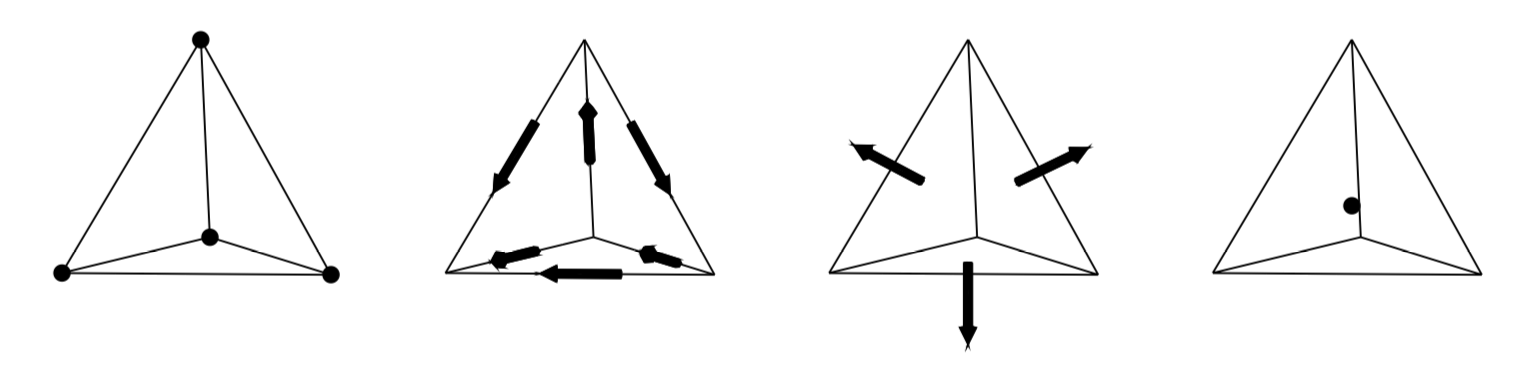
\includegraphics[height=2.5cm]{arnold}
      \end{center}
      \begin{flushright}
        \textcite{Arnold:2000} \hspace{4em}
      \end{flushright}
    \end{block}
  \end{onlyenv}

  \begin{onlyenv}<5>
    \begin{block}{An augmented Lagrangian approach to the Oseen problem}
      We use a block Gauss-Seidel method [...] based on the
      decomposition $V_h = \sum_{i=0}^l V_i$ [...For] P2-P0 finite
      elements the natural choice is to gather nodel DOFs for velocity
      inside ovals [around a vertex]

      \begin{center}
        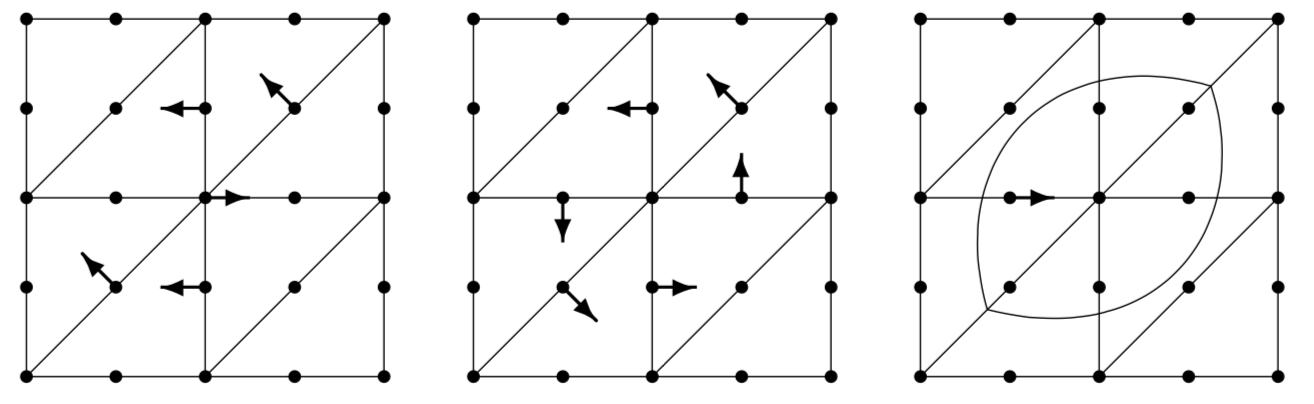
\includegraphics[height=2.5cm]{benzi}
      \end{center}
      \begin{flushright}
        \textcite{Benzi:2006} \hspace{4em}
      \end{flushright}
    \end{block}
  \end{onlyenv}
\end{frame}

\begin{frame}
  \frametitle{Unifying observation}
  \begin{block}{Abstract relaxation method}
    Choose a subspace decomposition
    \begin{equation*}
      V = \sum_i V_i
    \end{equation*}
    solve the problem on each subspace and combine the updates.
  \end{block}
  \begin{example}
    If $V_i$ is the span of a single basis function, then we have
    Jacobi or Gau\ss-Seidel relaxation (parallel or sequential
    subspace solves)
  \end{example}
  \begin{itemize}
  \item Decompose space (usually) based on some mesh decomposition
  \item Build and solve little problems on the resulting patches
  \item Combine additively or multiplicatively
  \end{itemize}
\end{frame}

\begin{frame}
  \frametitle{\texttt{PCPATCH}}
  \begin{block}{Topological decomposition}
    Use \texttt{DMPlex} to provide decomposition of mesh into patches.
  \end{block}

  \begin{block}{Space decomposition}
    Use topological decomposition plus \texttt{PetscSection} to
    determine degrees of freedom in each patch.
  \end{block}

  \begin{block}{Building patch problems}
    Callback interface to discretisation/PDE library.
  \end{block}
\end{frame}

\begin{frame}[t]
  \frametitle{DMPlex notation}
  Description of patches uses DMPlex nomenclature
  \begin{columns}[T]
    \begin{column}{0.4\textwidth}
      \begin{block}{Mesh}
        \begin{center}
          \begin{tikzpicture}
            \node (0) [nodraw, label=below:{\tettextsize 2}] at (0,0) {};
\node (1) [nodraw, label=below:{\tettextsize 3}] at (2.4,0) {};
\node (2) [nodraw, label=above right:{\tettextsize 4}] at (2.3,0.84) {};
\node (3) [nodraw, label=above:{\tettextsize 1}] at (1.2,2.0) {};

\path[line] (0) edge node[label=below:{\tettextsize 9}]{} (1);
%% \draw[line] (0) -- (1);
\path[line, dashed] (0) edge node[label=above:{\tettextsize 14}]{} (2);
\path[line] (1) edge node[label=right:{\tettextsize 12}]{} (2);
\draw[line] (0) edge node[label=above left:{\tettextsize 11}]{} (3);
\draw[line] (1) edge node[label=left:{\tettextsize 10}]{} (3);
\draw[line] (2) edge node[label=above right:{\tettextsize 13}]{} (3);

          \end{tikzpicture}
        \end{center}
      \end{block}
    \end{column}
    \begin{column}{0.6\textwidth}
      \begin{block}{Graph representation}
        \begin{onlyenv}<1>
          \begin{center}
            \begin{tikzpicture}
              \def\y{.79}
\def\x{.32}
\node (0) [cell] at (0,0) {0};
\node (1) [facet] at (-3*\x, \y) {5};
\node (2) [facet] at (-1*\x, \y) {6};
\node (3) [facet] at (1*\x, \y) {7};
\node (4) [facet] at (3*\x, \y) {8};
\node (5) [edge] at (-4*\x, 2*\y) {9};
\node (6) [edge] at (-2.4*\x, 2*\y) {10};
\node (7) [edge] at (-.8*\x, 2*\y) {11};
\node (8) [edge] at (.8*\x, 2*\y) {12};
\node (9) [edge] at (2.4*\x, 2*\y) {13};
\node (10) [edge] at (4*\x, 2*\y) {14};
\node (11) [vertex] at (-3*\x, 3*\y) {1};
\node (12) [vertex] at (-1*\x, 3*\y) {2};
\node (13) [vertex] at (1*\x, 3*\y) {3};
\node (14) [vertex] at (3*\x, 3*\y) {4};

\draw[line] (0) -- (1);
\draw[line] (0) -- (2);
\draw[line] (0) -- (3);
\draw[line] (0) -- (4);
\draw[line] (1) -- (5);
\draw[line] (1) -- (6);
\draw[line] (1) -- (7);
\draw[line] (2) -- (6);
\draw[line] (2) -- (8);
\draw[line] (2) -- (9);
\draw[line] (3) -- (7);
\draw[line] (3) -- (9);
\draw[line] (3) -- (10);
\draw[line] (4.north west) -- (5.south east);
\draw[line] (4) -- (8);
\draw[line] (4) -- (10);
\draw[line] (5) -- (12);
\draw[line] (5) -- (13);
\draw[line] (6) -- (11);
\draw[line] (6) -- (13);
\draw[line] (7) -- (11);
\draw[line] (7) -- (12);
\draw[line] (8) -- (13);
\draw[line] (8) -- (14);
\draw[line] (9) -- (11);
\draw[line] (9) -- (14);
\draw[line] (10) -- (12);
\draw[line] (10) -- (14);

            \end{tikzpicture}
          \end{center}
        \end{onlyenv}
        \begin{onlyenv}<2>
          \begin{center}
            \begin{tikzpicture}
              \def\y{.79}
\def\x{.32}
\node (0) [cell] at (0,0) {0};
\node (1) [facet] at (-3*\x, \y) {5};
\node (2) [facet] at (-1*\x, \y) {6};
\node (3) [facet] at (1*\x, \y) {7};
\node (4) [facet] at (3*\x, \y) {8};
\node (5) [edge] at (-4*\x, 2*\y) {9};
\node (6) [edge] at (-2.4*\x, 2*\y) {10};
\node (7) [edge] at (-.8*\x, 2*\y) {11};
\node (8) [edge] at (.8*\x, 2*\y) {12};
\node (9) [edge] at (2.4*\x, 2*\y) {13};
\node (10) [edge] at (4*\x, 2*\y) {14};
\node (11) [vertex] at (-3*\x, 3*\y) {1};
\node (12) [vertex] at (-1*\x, 3*\y) {2};
\node (13) [vertex] at (1*\x, 3*\y) {3};
\node (14) [vertex] at (3*\x, 3*\y) {4};

\draw[line] (0) -- (1);
\draw[line] (0) -- (2);
\draw[line] (0) -- (3);
\draw[line] (0) -- (4);
\draw[line] (1) -- (5);
\draw[line] (1) -- (6);
\draw[line] (1) -- (7);
\draw[line] (2) -- (6);
\draw[line] (2) -- (8);
\draw[line] (2) -- (9);
\draw[line] (3) -- (7);
\draw[line] (3) -- (9);
\draw[line] (3) -- (10);
\draw[line] (4.north west) -- (5.south east);
\draw[line] (4) -- (8);
\draw[line] (4) -- (10);
\draw[line] (5) -- (12);
\draw[line] (5) -- (13);
\draw[line] (6) -- (11);
\draw[line] (6) -- (13);
\draw[line] (7) -- (11);
\draw[line] (7) -- (12);
\draw[line] (8) -- (13);
\draw[line] (8) -- (14);
\draw[line] (9) -- (11);
\draw[line] (9) -- (14);
\draw[line] (10) -- (12);
\draw[line] (10) -- (14);

              \begin{scope}[overlay, remember picture, rounded corners]
                \filldraw[fill opacity=0.2]
                ([xshift= 3pt, yshift=-3pt] 7.south east) --
                ([xshift= 3pt, yshift= 3pt] 7.north east) --
                ([xshift=-3pt, yshift= 3pt] 5.north west) --
                ([xshift=-3pt, yshift=-3pt] 5.south west) --
                cycle;
                \node[cell, fill=black, opacity=0.6] at (1.center) {};
              \end{scope}
            \end{tikzpicture}
          \end{center}
          $\text{\texttt{cone}}(5) = \{9, 10, 11\}$
        \end{onlyenv}
        \begin{onlyenv}<3>
          \begin{center}
            \begin{tikzpicture}
              \def\y{.79}
\def\x{.32}
\node (0) [cell] at (0,0) {0};
\node (1) [facet] at (-3*\x, \y) {5};
\node (2) [facet] at (-1*\x, \y) {6};
\node (3) [facet] at (1*\x, \y) {7};
\node (4) [facet] at (3*\x, \y) {8};
\node (5) [edge] at (-4*\x, 2*\y) {9};
\node (6) [edge] at (-2.4*\x, 2*\y) {10};
\node (7) [edge] at (-.8*\x, 2*\y) {11};
\node (8) [edge] at (.8*\x, 2*\y) {12};
\node (9) [edge] at (2.4*\x, 2*\y) {13};
\node (10) [edge] at (4*\x, 2*\y) {14};
\node (11) [vertex] at (-3*\x, 3*\y) {1};
\node (12) [vertex] at (-1*\x, 3*\y) {2};
\node (13) [vertex] at (1*\x, 3*\y) {3};
\node (14) [vertex] at (3*\x, 3*\y) {4};

\draw[line] (0) -- (1);
\draw[line] (0) -- (2);
\draw[line] (0) -- (3);
\draw[line] (0) -- (4);
\draw[line] (1) -- (5);
\draw[line] (1) -- (6);
\draw[line] (1) -- (7);
\draw[line] (2) -- (6);
\draw[line] (2) -- (8);
\draw[line] (2) -- (9);
\draw[line] (3) -- (7);
\draw[line] (3) -- (9);
\draw[line] (3) -- (10);
\draw[line] (4.north west) -- (5.south east);
\draw[line] (4) -- (8);
\draw[line] (4) -- (10);
\draw[line] (5) -- (12);
\draw[line] (5) -- (13);
\draw[line] (6) -- (11);
\draw[line] (6) -- (13);
\draw[line] (7) -- (11);
\draw[line] (7) -- (12);
\draw[line] (8) -- (13);
\draw[line] (8) -- (14);
\draw[line] (9) -- (11);
\draw[line] (9) -- (14);
\draw[line] (10) -- (12);
\draw[line] (10) -- (14);

              \begin{scope}[overlay, remember picture, rounded corners]
                \filldraw[fill opacity=0.2]
                ([xshift= 1pt, yshift=-3pt] 1.south east) --
                ([xshift=-3pt, yshift= 1pt] 2.north west) --
                ([xshift= 3pt, yshift=-1pt] 7.south east) --
                ([xshift=-3pt, yshift= 1pt] 8.north west) --
                ([xshift= 3pt, yshift=-1pt] 13.south east) --
                ([xshift= 3pt, yshift= 3pt] 13.north east) --
                ([xshift=-2pt, yshift= 3pt] 11.north west) --
                ([xshift=-2pt, yshift= 0pt] 5.west) --
                ([xshift=-1pt, yshift=-3pt] 1.south west) --
                cycle;
                \node[cell, fill=black, opacity=0.6] at (1.center) {};
              \end{scope}
            \end{tikzpicture}
          \end{center}
          $\text{\texttt{closure}}(5) = \{1, 2, 3, 9, 10, 11\}$
        \end{onlyenv}
        \begin{onlyenv}<4>
          \begin{center}
            \begin{tikzpicture}
              \def\y{.79}
\def\x{.32}
\node (0) [cell] at (0,0) {0};
\node (1) [facet] at (-3*\x, \y) {5};
\node (2) [facet] at (-1*\x, \y) {6};
\node (3) [facet] at (1*\x, \y) {7};
\node (4) [facet] at (3*\x, \y) {8};
\node (5) [edge] at (-4*\x, 2*\y) {9};
\node (6) [edge] at (-2.4*\x, 2*\y) {10};
\node (7) [edge] at (-.8*\x, 2*\y) {11};
\node (8) [edge] at (.8*\x, 2*\y) {12};
\node (9) [edge] at (2.4*\x, 2*\y) {13};
\node (10) [edge] at (4*\x, 2*\y) {14};
\node (11) [vertex] at (-3*\x, 3*\y) {1};
\node (12) [vertex] at (-1*\x, 3*\y) {2};
\node (13) [vertex] at (1*\x, 3*\y) {3};
\node (14) [vertex] at (3*\x, 3*\y) {4};

\draw[line] (0) -- (1);
\draw[line] (0) -- (2);
\draw[line] (0) -- (3);
\draw[line] (0) -- (4);
\draw[line] (1) -- (5);
\draw[line] (1) -- (6);
\draw[line] (1) -- (7);
\draw[line] (2) -- (6);
\draw[line] (2) -- (8);
\draw[line] (2) -- (9);
\draw[line] (3) -- (7);
\draw[line] (3) -- (9);
\draw[line] (3) -- (10);
\draw[line] (4.north west) -- (5.south east);
\draw[line] (4) -- (8);
\draw[line] (4) -- (10);
\draw[line] (5) -- (12);
\draw[line] (5) -- (13);
\draw[line] (6) -- (11);
\draw[line] (6) -- (13);
\draw[line] (7) -- (11);
\draw[line] (7) -- (12);
\draw[line] (8) -- (13);
\draw[line] (8) -- (14);
\draw[line] (9) -- (11);
\draw[line] (9) -- (14);
\draw[line] (10) -- (12);
\draw[line] (10) -- (14);

              \begin{scope}[overlay, remember picture, rounded corners]
                \filldraw[fill opacity=0.2]
                ([xshift= 3pt, yshift=-3pt] 10.south east) --
                ([xshift= 3pt, yshift= 3pt] 10.north east) --
                ([xshift=-3pt, yshift= 3pt] 8.north west) --
                ([xshift=-3pt, yshift=-3pt] 8.south west) --
                cycle;
                \node[cell, fill=black, opacity=0.6] at (14.center) {};
              \end{scope}
            \end{tikzpicture}
          \end{center}
          $\text{\texttt{support}}(4) = \{12, 13, 14\}$
        \end{onlyenv}
        \begin{onlyenv}<5>
          \begin{center}
            \begin{tikzpicture}
              \def\y{.79}
\def\x{.32}
\node (0) [cell] at (0,0) {0};
\node (1) [facet] at (-3*\x, \y) {5};
\node (2) [facet] at (-1*\x, \y) {6};
\node (3) [facet] at (1*\x, \y) {7};
\node (4) [facet] at (3*\x, \y) {8};
\node (5) [edge] at (-4*\x, 2*\y) {9};
\node (6) [edge] at (-2.4*\x, 2*\y) {10};
\node (7) [edge] at (-.8*\x, 2*\y) {11};
\node (8) [edge] at (.8*\x, 2*\y) {12};
\node (9) [edge] at (2.4*\x, 2*\y) {13};
\node (10) [edge] at (4*\x, 2*\y) {14};
\node (11) [vertex] at (-3*\x, 3*\y) {1};
\node (12) [vertex] at (-1*\x, 3*\y) {2};
\node (13) [vertex] at (1*\x, 3*\y) {3};
\node (14) [vertex] at (3*\x, 3*\y) {4};

\draw[line] (0) -- (1);
\draw[line] (0) -- (2);
\draw[line] (0) -- (3);
\draw[line] (0) -- (4);
\draw[line] (1) -- (5);
\draw[line] (1) -- (6);
\draw[line] (1) -- (7);
\draw[line] (2) -- (6);
\draw[line] (2) -- (8);
\draw[line] (2) -- (9);
\draw[line] (3) -- (7);
\draw[line] (3) -- (9);
\draw[line] (3) -- (10);
\draw[line] (4.north west) -- (5.south east);
\draw[line] (4) -- (8);
\draw[line] (4) -- (10);
\draw[line] (5) -- (12);
\draw[line] (5) -- (13);
\draw[line] (6) -- (11);
\draw[line] (6) -- (13);
\draw[line] (7) -- (11);
\draw[line] (7) -- (12);
\draw[line] (8) -- (13);
\draw[line] (8) -- (14);
\draw[line] (9) -- (11);
\draw[line] (9) -- (14);
\draw[line] (10) -- (12);
\draw[line] (10) -- (14);

              \begin{scope}[overlay, remember picture, rounded corners]
                \filldraw[fill opacity=0.2]
                ([xshift= 0pt, yshift= 3pt] 14.north west) --
                ([xshift= 3pt, yshift=-3pt] 13.south east) --
                ([xshift=-3pt, yshift= 1pt] 8.north west) --
                ([xshift= 3pt, yshift=-1pt] 7.south east) --
                ([xshift=-3pt, yshift= 1pt] 2.north west) --
                ([xshift=-3pt, yshift= 1pt] 2.south west) --
                ([xshift= 0pt, yshift=-3pt] 0.south west) --
                ([xshift= 0pt, yshift=-3pt] 0.south east) --
                ([xshift= 3pt, yshift=-1pt] 4.south east) --
                ([xshift= 3pt, yshift= 0pt] 10.east) --
                ([xshift= 2pt, yshift= 3pt] 14.north east) --
                cycle;
                \node[cell, fill=black, opacity=0.6] at (14.center) {};
              \end{scope}
            \end{tikzpicture}
          \end{center}
          $\text{\texttt{star}}(4) = \{0, 6, 7, 8, 12, 13, 14\}$
        \end{onlyenv}
      \end{block}
    \end{column}
  \end{columns}
\end{frame}

\begin{frame}[fragile]
 \frametitle{Topological subspace definition via \texttt{DMPlex}}
 \begin{itemize}
 \item Each patch defined by set of mesh points (entities) on which the dofs
   we're going to solve for in the patch live
 \end{itemize}
 \begin{block}{Builtin}
   Specify patches by selecting:
   \begin{enumerate}
   \item Mesh points $\{p_i\}$ to iterate over (e.g.~vertices, cells)
   \item Adjacency relation that gathers points in patch
     \begin{itemize}
     \item[\texttt{star}] points in $\text{star}(p_i)$
     \item[\texttt{vanka}] points in $\text{closure}(\text{star}(p_i))$
     \end{itemize}
   \end{enumerate}
 \end{block}
 \begin{block}{User-defined}
   Callback provides \texttt{IS}es for each patch, plus iteration order.
\begin{minted}[fontsize=\scriptsize]{c}
 PetscErrorCode UserPatches(PC, PetscInt *npatch, IS **patches,
                            IS *order, void *ctx);
\end{minted}
 \end{block}
\end{frame}

\begin{frame}
  \frametitle{Connect to dofs via \texttt{PetscSection}}
  \begin{itemize}
  \item Each patch defined by set of mesh points $\{p_i\}$
  \item Inspect \texttt{PetscSection} defining the function space
    layout to obtain global dof numbers
  \item These are the dofs we will solve for
  \item Create local renumbering on each patch (for local operator)
  \item Build scatters from global to patch vectors
  \item Finally, \emph{complete} patch using appropriate adjacency
    relationship (this pulls in dofs we need to see, but will not
    solve for)
  \end{itemize}
\end{frame}
\begin{frame}[fragile,t]
  \frametitle{Patch assembly}
  \begin{itemize}
  \item If we only want homogeneous Dirichlet, can use list of dofs to
    select from assembled global operator
  \item Other transmission conditions this doesn't work
  \item Instead, callback interface
  \item Extends to \emph{nonlinear} smoothers
  \end{itemize}

  \begin{onlyenv}<1>
    \begin{block}{Callbacks}
\begin{minted}[fontsize=\scriptsize]{c}
 /* Patch Jacobian */
 UserComputeOp(PC, PetscInt point, Vec state, Mat op, IS cells,
               PetscInt n, PetscInt *dofmap, void *ctx);
 /* Patch Residual */
 UserComputeF(PC, PetscInt point, Vec state, Vec f, IS cells,
              PetscInt n, PetscInt *dofmapWithBcs, PetscInt *dofmap,
              void *ctx);
\end{minted}
    \end{block}
  \end{onlyenv}
  \begin{onlyenv}<2>
    \begin{block}{PDE library support}
      \begin{itemize}
      \item Works if you use \texttt{DMPlex} + \texttt{PetscDS}
\begin{minted}[fontsize=\scriptsize]{sh}
-pc_type patch
\end{minted}
      \item Works in Firedrake
\begin{minted}[fontsize=\scriptsize]{sh}
-pc_type python -pc_python_type firedrake.PatchPC
# Also
-snes_type python -snes_python_type firedrake.PatchSNES
\end{minted}
      \end{itemize}
    \end{block}
  \end{onlyenv}
\end{frame}

\section{Examples}

\begin{frame}
  \frametitle{What subspace to choose?}
  \begin{onlyenv}<1> Consider the problem: for
    $\alpha, \beta \in \mathbb{R}$, find $u \in V$ such that
    \begin{equation*}
      \alpha a(u, v) + \beta b(u, v) = (f, v) \quad \forall v \in V,
    \end{equation*}
    where $a$ is SPD, and $b$ is symmetric positive semidefinite.
  \end{onlyenv}
  \begin{theorem}[Sch\"oberl (1999); Lee, Wu, Xu, Zikatanov (2007)]
    Let the kernel be
    \begin{equation*}
      \mathcal{N} := \{ u \in V : b(u, v) = 0 \,\, \forall v \in V \}.
    \end{equation*}
    If the subspace decomposition \emph{captures the kernel}
    \begin{equation*}
      \mathcal{N} = \sum_i \mathcal{N} \cap V_i,
    \end{equation*}
    then convergence of the relaxation defined by this decomposition
    will be \emph{independent} of $\alpha$ and $\beta$.
    \nocite{Schoeberl:1999,Lee:2007}
  \end{theorem}
  \begin{onlyenv}<2>
    \begin{corollary}
      ``All'' we need to do is find a basis for the kernel.

      Appropriate discrete de Rham complexes can help.
    \end{corollary}
  \end{onlyenv}
\end{frame}

\begin{frame}[fragile]
  \frametitle{Nearly incompressible elasticity}
  \vspace*{-1.5\baselineskip}
  \begin{equation*}
    \text{Find $u \in V \subset H^1$ s.t.} \quad (\grad u, \grad v) + \gamma (\div u, \div v) = (f, v) \quad \forall v \in V.
  \end{equation*}
  \vspace*{-\baselineskip}
  \begin{block}{Stokes complex}
    \begin{equation*}
      \mathbb{R} \xrightarrow{\operatorname{id}} H^2 \xrightarrow{\grad} H^1(\curl)
      \xrightarrow{\curl} H^1 \xrightarrow{\div} L^2 \xrightarrow{\operatorname{null}} 0,
    \end{equation*}
    Decomposition must span $\ker \div = \range \curl$.

    Appropriate discrete spaces are constructed in \textcite{Neilan:2015a}: use
    star patch around vertices (with piecewise continuous space for
    $H^1$ of sufficiently high degree).
  \end{block}
  \begin{onlyenv}<1-3>
    \begin{columns}
      \begin{column}{0.6\textwidth}
        \begin{onlyenv}<1>
\begin{minted}[fontsize=\scriptsize]{python}
-ksp_type cg
-pc_type mg
-mg_levels_
   -pc_type python
   -pc_python_type firedrake.PatchPC
   -patch_


\end{minted}
        \end{onlyenv}
        \begin{onlyenv}<2>
\begin{minted}[fontsize=\scriptsize]{python}
-ksp_type cg
-pc_type mg
-mg_levels_
   -pc_type python
   -pc_python_type firedrake.PatchPC
   -patch_
      -pc_patch_construct_dim 0

\end{minted}
        \end{onlyenv}
        \begin{onlyenv}<3>
\begin{minted}[fontsize=\scriptsize]{python}
-ksp_type cg
-pc_type mg
-mg_levels_
   -pc_type python
   -pc_python_type firedrake.PatchPC
   -patch_
      -pc_patch_construct_dim 0
      -pc_patch_construct_type star
\end{minted}
        \end{onlyenv}
      \end{column}
      \begin{column}{0.4\textwidth}
        \begin{center}
          \begin{tikzpicture}[scale=4]
            \tikzstyle{v}=[circle, fill, minimum size=0pt, inner sep=0pt]
            \tikzstyle{c}=[diamond, fill, minimum size=4pt, inner sep=0pt]
            \tikzstyle{e}=[rectangle, fill, minimum size=3pt, inner sep=0pt]
            \tikzstyle{select}=[draw, minimum size=3pt]
            \foreach \i/\k in {0/0, 0.25/1, 0.5/2, 0.75/3} {
              \foreach \j/\l in {0/0, 0.25/1, 0.5/2, 0.75/3} {
                \node[v] (v\k\l) at (\i, \j) {};
              }
            }

            \foreach \i in {0, 0.25, 0.5, 0.75} {
              \foreach \j/\k in {0/0.25, 0.25/0.5, 0.5/0.75} {
                \draw[thin, gray] (\i, \j) -- (\i, \k);
                \draw[thin, gray] (\j, \i) -- (\k, \i);
              }
            }
            \foreach \i/\j in {0/0.25, 0.25/0.5, 0.5/0.75} {
              \foreach \k/\l in {0/0.25, 0.25/0.5, 0.5/0.75} {
                \draw[thin, gray] (\i, \l) -- (\j, \k);
              }
            }

            \uncover<2-3>{
              \node[v, select] at (v11) {};
              \node[v, select] at (v21) {};
              \node[v, select] at (v12) {};
              \node[v, select] at (v22) {};
            }
            \foreach \a/\b in {0/1, 1/2, 2/3} {
              \foreach \c/\d in {1/0, 2/1, 3/2} {
                \node (c\a\c-\b\c-\b\d) at (barycentric cs:v\a\c=1,v\b\c=1,v\b\d=1) {};
                \node (c\a\d-\b\d-\a\c) at (barycentric cs:v\a\d=1,v\b\d=1,v\a\c=1) {};
              }
            }

            \uncover<3>{
              \draw[thick] \convexpath{
                c02-12-11,
                c11-21-12,
                c11-21-20,
                c10-20-11,
                c01-11-10,
                c01-11-02}{1pt};
              \draw[thick] \convexpath{
                c12-22-21,
                c21-31-22,
                c21-31-30,
                c20-30-21,
                c11-21-20,
                c11-21-12}{1pt};
              \draw[thick] \convexpath{
                c03-13-12,
                c12-22-13,
                c12-22-21,
                c11-21-12,
                c02-12-11,
                c02-12-03}{1pt};
              \draw[thick] \convexpath{
                c13-23-22,
                c22-32-23,
                c22-32-31,
                c21-31-22,
                c12-22-21,
                c12-22-13}{1pt};
            }
          \end{tikzpicture}
        \end{center}
      \end{column}
    \end{columns}
  \end{onlyenv}
  \begin{onlyenv}<4>
    \begin{table}
      \centering
      {\footnotesize
      \begin{tabular}{l|cccccc}
        $k\backslash \gamma$ & $10^0$ & $10^1$ & $10^2$ & $10^3$ & $10^4$ & $10^5$ \\
        \hline
        3                    & 11     & 16     & 29     & 66     & 173    & 458    \\
        4                    & 11     & 13     & 19     & 26     & 54     & 110    \\
        5                    & 11     & 12     & 16     & 19     & 20     & 19     \\
        6                    & 10     & 11     & 14     & 15     & 16     & 15     \\
        7                    & 10     & 11     & 13     & 14     & 14     & 13     \\
      \end{tabular}
      \caption{Convergence with vertex star patch preconditioned Richardson
        smoothers and $P_k$ Lagrange elements}
      }
    \end{table}
  \end{onlyenv}
\end{frame}

\begin{frame}[fragile]
  \frametitle{H(div) Riesz map}
  \vspace{-1.5\baselineskip}
  \begin{equation*}
    \text{Find $u \in V \subset H(\div)$ s.t.}\quad (u, v) + \gamma (\div u, \div v) = (f, v) \quad \forall v \in V.
  \end{equation*}
  \vspace*{-\baselineskip}
  \begin{block}{Whitney-N\'ed\'elec complex}
    \begin{equation*}
      \mathbb{R} \xrightarrow{\operatorname{id}} H^1 \xrightarrow{\grad} H(\curl)
      \xrightarrow{\curl} H(\div) \xrightarrow{\div} L^2 \xrightarrow{\operatorname{null}} 0,
    \end{equation*}
    Decomposition must span $\ker \div = \range \curl$.

    Choose $V$ to be a Raviart-Thomas space, the matching $H(\curl)$
    space has dofs on edges: use star patch around edges.
  \end{block}
  \begin{onlyenv}<1-3>
    \begin{columns}
      \begin{column}{0.6\textwidth}
        \begin{onlyenv}<1>
\begin{minted}[fontsize=\scriptsize]{python}
-ksp_type cg
-pc_type mg
-mg_levels_
   -pc_type python
   -pc_python_type firedrake.PatchPC
   -patch_


\end{minted}
        \end{onlyenv}
        \begin{onlyenv}<2>
\begin{minted}[fontsize=\scriptsize]{python}
-ksp_type cg
-pc_type mg
-mg_levels_
   -pc_type python
   -pc_python_type firedrake.PatchPC
   -patch_
      -pc_patch_construct_dim 1

\end{minted}
        \end{onlyenv}
        \begin{onlyenv}<3>
\begin{minted}[fontsize=\scriptsize]{python}
-ksp_type cg
-pc_type mg
-mg_levels_
   -pc_type python
   -pc_python_type firedrake.PatchPC
   -patch_
      -pc_patch_construct_dim 1
      -pc_patch_construct_type star
\end{minted}
        \end{onlyenv}
      \end{column}
      \begin{column}{0.4\textwidth}
        \begin{center}
          \begin{tikzpicture}[scale=4]
            \tikzstyle{v}=[circle, fill, minimum size=0pt, inner sep=0pt]
            \tikzstyle{c}=[diamond, fill, minimum size=4pt, inner sep=0pt]
            \tikzstyle{e}=[rectangle, fill, minimum size=3pt, inner sep=0pt]
            \tikzstyle{select}=[draw, minimum size=3pt]
            \foreach \i/\k in {0/0, 0.25/1, 0.5/2, 0.75/3} {
              \foreach \j/\l in {0/0, 0.25/1, 0.5/2, 0.75/3} {
                \node[v] (v\k\l) at (\i, \j) {};
              }
            }

            \foreach \i in {0, 0.25, 0.5, 0.75} {
              \foreach \j/\k in {0/0.25, 0.25/0.5, 0.5/0.75} {
                \draw[thin, gray] (\i, \j) -- (\i, \k);
                \draw[thin, gray] (\j, \i) -- (\k, \i);
              }
            }
            \foreach \i/\j in {0/0.25, 0.25/0.5, 0.5/0.75} {
              \foreach \k/\l in {0/0.25, 0.25/0.5, 0.5/0.75} {
                \draw[thin, gray] (\i, \l) -- (\j, \k);
              }
            }
            \foreach \a/\b in {0/1, 1/2, 2/3} {
              \foreach \c/\d in {1/0, 2/1, 3/2} {
                \node (c\a\c-\b\c-\b\d) at (barycentric cs:v\a\c=1,v\b\c=1,v\b\d=1) {};
                \node (c\a\d-\b\d-\a\c) at (barycentric cs:v\a\d=1,v\b\d=1,v\a\c=1) {};
              }
            }
            \node (e1) at (barycentric cs:v12=1,v22=2) {};
            \node (e2) at (barycentric cs:v12=2,v22=1) {};

            \node (e3) at (barycentric cs:v11=1,v21=2) {};
            \node (e4) at (barycentric cs:v11=2,v21=1) {};

            \node (e5) at (barycentric cs:v21=1,v12=2) {};
            \node (e6) at (barycentric cs:v21=2,v12=1) {};

            \uncover<2-3>{
              \node[e, select] at (barycentric cs:v12=1,v22=1) {};
              \node[e, select] at (barycentric cs:v11=1,v21=1) {};
              \node[e, select] at (barycentric cs:v21=1,v12=1) {};
            }

            \uncover<3>{
              \draw[thick] \convexpath{
                c12-22-13,
                e1,
                c12-22-21,
                e2}{1pt};

              \draw[thick] \convexpath{
                c11-21-12,
                e3,
                c11-21-20,
                e4}{1pt};

              \draw[thick] \convexpath{
                c11-21-12,
                e5,
                c12-22-21,
                e6}{1pt};
            }
          \end{tikzpicture}
        \end{center}
      \end{column}
    \end{columns}
  \end{onlyenv}
  \begin{onlyenv}<4>
    \begin{table}
      \centering
      {\footnotesize
      \begin{tabular}{l|cccccc}
        $k\backslash \gamma$ & $10^0$ & $10^1$ & $10^2$ & $10^3$ & $10^4$ & $10^5$ \\
        \hline
        1 (vertex)           & 11     & 11     & 11     & 11     & 11     & 11     \\
        2 (vertex)           & 7      & 7      & 7      & 7      & 7      & 7      \\
        1 (edge)             & 32     & 32     & 32     & 32     & 32     & 32     \\
        2 (edge)             & 15     & 15     & 15     & 15     & 15     & 15     \\
      \end{tabular}
      \caption{Convergence with vertex and edge star patch preconditioned Richardson
        smoothers and $\text{RT}_k$ elements}
      }
    \end{table}
  \end{onlyenv}
\end{frame}

\begin{frame}[fragile]
  \frametitle{H(curl) Riesz map}
  \vspace{-1.5\baselineskip}
  \begin{equation*}
    \text{  Find $u \in V \subset H(\curl)$ s.t.} \quad (u, v) + \gamma (\curl u, \curl v) = (f, v) \quad \forall v \in V.
  \end{equation*}
  \vspace{-\baselineskip}
  \begin{block}{Whitney-N\'ed\'elec complex}
    \begin{equation*}
      \mathbb{R} \xrightarrow{\operatorname{id}} H^1 \xrightarrow{\grad} H(\curl)
      \xrightarrow{\curl} H(\div) \xrightarrow{\div} L^2 \xrightarrow{\operatorname{null}} 0,
    \end{equation*}
    Decomposition must span $\ker \curl = \range \grad$.

    Choose $V$ to be a N\'ed\'elec space, the matching $H^1$
    space has dofs at vertices: use star patch around vertices.
  \end{block}
  \begin{onlyenv}<1-3>
    \begin{columns}
      \begin{column}{0.6\textwidth}
        \begin{onlyenv}<1>
\begin{minted}[fontsize=\scriptsize]{python}
-ksp_type cg
-pc_type mg
-mg_levels_
   -pc_type python
   -pc_python_type firedrake.PatchPC
   -patch_


\end{minted}
        \end{onlyenv}
        \begin{onlyenv}<2>
\begin{minted}[fontsize=\scriptsize]{python}
-ksp_type cg
-pc_type mg
-mg_levels_
   -pc_type python
   -pc_python_type firedrake.PatchPC
   -patch_
      -pc_patch_construct_dim 0

\end{minted}
        \end{onlyenv}
        \begin{onlyenv}<3>
\begin{minted}[fontsize=\scriptsize]{python}
-ksp_type cg
-pc_type mg
-mg_levels_
   -pc_type python
   -pc_python_type firedrake.PatchPC
   -patch_
      -pc_patch_construct_dim 0
      -pc_patch_construct_type star
\end{minted}
        \end{onlyenv}
      \end{column}
      \begin{column}{0.4\textwidth}
        \begin{center}
          \begin{tikzpicture}[scale=4]
            \tikzstyle{v}=[circle, fill, minimum size=0pt, inner sep=0pt]
            \tikzstyle{c}=[diamond, fill, minimum size=4pt, inner sep=0pt]
            \tikzstyle{e}=[rectangle, fill, minimum size=3pt, inner sep=0pt]
            \tikzstyle{select}=[draw, minimum size=3pt]
            \foreach \i/\k in {0/0, 0.25/1, 0.5/2, 0.75/3} {
              \foreach \j/\l in {0/0, 0.25/1, 0.5/2, 0.75/3} {
                \node[v] (v\k\l) at (\i, \j) {};
              }
            }

            \foreach \i in {0, 0.25, 0.5, 0.75} {
              \foreach \j/\k in {0/0.25, 0.25/0.5, 0.5/0.75} {
                \draw[thin, gray] (\i, \j) -- (\i, \k);
                \draw[thin, gray] (\j, \i) -- (\k, \i);
              }
            }
            \foreach \i/\j in {0/0.25, 0.25/0.5, 0.5/0.75} {
              \foreach \k/\l in {0/0.25, 0.25/0.5, 0.5/0.75} {
                \draw[thin, gray] (\i, \l) -- (\j, \k);
              }
            }

            \uncover<2-3>{
              \node[v, select] at (v11) {};
              \node[v, select] at (v21) {};
              \node[v, select] at (v12) {};
              \node[v, select] at (v22) {};
            }
            \foreach \a/\b in {0/1, 1/2, 2/3} {
              \foreach \c/\d in {1/0, 2/1, 3/2} {
                \node (c\a\c-\b\c-\b\d) at (barycentric cs:v\a\c=1,v\b\c=1,v\b\d=1) {};
                \node (c\a\d-\b\d-\a\c) at (barycentric cs:v\a\d=1,v\b\d=1,v\a\c=1) {};
              }
            }

            \uncover<3>{
              \draw[thick] \convexpath{
                c02-12-11,
                c11-21-12,
                c11-21-20,
                c10-20-11,
                c01-11-10,
                c01-11-02}{1pt};
              \draw[thick] \convexpath{
                c12-22-21,
                c21-31-22,
                c21-31-30,
                c20-30-21,
                c11-21-20,
                c11-21-12}{1pt};
              \draw[thick] \convexpath{
                c03-13-12,
                c12-22-13,
                c12-22-21,
                c11-21-12,
                c02-12-11,
                c02-12-03}{1pt};
              \draw[thick] \convexpath{
                c13-23-22,
                c22-32-23,
                c22-32-31,
                c21-31-22,
                c12-22-21,
                c12-22-13}{1pt};
            }
          \end{tikzpicture}
        \end{center}
      \end{column}
    \end{columns}
  \end{onlyenv}
  \begin{onlyenv}<4>
    \begin{table}
      \centering
      {\footnotesize
      \begin{tabular}{l|cccccc}
        $k\backslash \gamma$ & $10^0$ & $10^1$ & $10^2$ & $10^3$ & $10^4$ & $10^5$ \\
        \hline
        1                    & 13     & 13     & 13     & 13     & 13     & 13     \\
        2                    & 10     & 10     & 10     & 10     & 10     & 10     \\
      \end{tabular}
      \caption{Convergence with vertex star patch preconditioned Richardson
        smoothers and $\text{N1curl}_k$ elements}
      }
    \end{table}
  \end{onlyenv}
\end{frame}

\begin{frame}[fragile, t]
  \frametitle{Vanka for Stokes}
  Find $(u, p) \in V\times Q \subset (H^1)^d \times L^2$ s.t.
  \begin{equation*}
    (\grad u, \grad v) - (p, \div v) - (\div u, q) = (f, v) \quad \forall (v, q) \in V \times Q.
  \end{equation*}

  \begin{block}{Vanka patch}
    Solve simultaneously for $(u, p)$ on each pressure dof, gathering
    those velocity dofs that couple to the pressure dof.

    \only<1-3>{Marker-and-Cell: loop over cells, gather closure of star}

    \only<4-7>{Taylor-Hood: loop over vertices, gather closure of star}
    \nocite{Vanka:1986}
  \end{block}
  \begin{onlyenv}<1-6>
    \begin{columns}
      \begin{column}{0.4\textwidth}
        \begin{onlyenv}<1-3>
          \begin{center}
            \begin{tikzpicture}[scale=4]
              \tikzstyle{v}=[circle, fill, minimum size=0pt, inner sep=0pt]
              \tikzstyle{c}=[diamond, fill, minimum size=4pt, inner sep=0pt]
              \tikzstyle{e}=[rectangle, fill, minimum size=3pt, inner sep=0pt]
              \tikzstyle{select}=[draw, minimum size=3pt]
              \foreach \i/\k in {0/0, 0.25/1, 0.5/2, 0.75/3} {
                \foreach \j/\l in {0/0, 0.25/1, 0.5/2, 0.75/3} {
                  \node[v] (v\k\l) at (\i, \j) {};
                }
              }

              \foreach \i in {0, 0.25, 0.5, 0.75} {
                \foreach \j/\k in {0/0.25, 0.25/0.5, 0.5/0.75} {
                  \draw[thin, gray] (\i, \j) -- (\i, \k);
                  \draw[thin, gray] (\j, \i) -- (\k, \i);
                }
              }
              \foreach \i/\j in {0/0.25, 0.25/0.5, 0.5/0.75} {
                \foreach \k/\l in {0/0.25, 0.25/0.5, 0.5/0.75} {
                  \draw[thin, gray] (\i, \l) -- (\j, \k);
                }
              }
              \foreach \a/\b in {0/1, 1/2, 2/3} {
                \foreach \c/\d in {1/0, 2/1, 3/2} {
                  \node (c\a\c-\b\c-\b\d) at (barycentric cs:v\a\c=1,v\b\c=1,v\b\d=1) {};
                  \node (c\a\d-\b\d-\a\c) at (barycentric cs:v\a\d=1,v\b\d=1,v\a\c=1) {};
                }
              }
              \uncover<2-3>{
                \node[c, select] at (c12-22-21) {};
                \node[c, select] at (c02-12-11) {};
                \node[c, select] at (c11-21-12) {};
              }
              \uncover<3>{
                \draw[thick] \convexpath{v02,v12,v11}{1pt};
                \draw[thick] \convexpath{v12,v21,v11}{1pt};
                \draw[thick] \convexpath{v12,v22,v21}{1pt};
              }
            \end{tikzpicture}
          \end{center}
        \end{onlyenv}
        \begin{onlyenv}<4-6>
          \begin{center}
            \begin{tikzpicture}[scale=4]
              \tikzstyle{v}=[circle, fill, minimum size=0pt, inner sep=0pt]
              \tikzstyle{c}=[diamond, fill, minimum size=4pt, inner sep=0pt]
              \tikzstyle{e}=[rectangle, fill, minimum size=3pt, inner sep=0pt]
              \tikzstyle{select}=[draw, minimum size=3pt]
              \foreach \i/\k in {0/0, 0.25/1, 0.5/2, 0.75/3} {
                \foreach \j/\l in {0/0, 0.25/1, 0.5/2, 0.75/3} {
                  \node[v] (v\k\l) at (\i, \j) {};
                }
              }

              \foreach \i in {0, 0.25, 0.5, 0.75} {
                \foreach \j/\k in {0/0.25, 0.25/0.5, 0.5/0.75} {
                  \draw[thin, gray] (\i, \j) -- (\i, \k);
                  \draw[thin, gray] (\j, \i) -- (\k, \i);
                }
              }
              \foreach \i/\j in {0/0.25, 0.25/0.5, 0.5/0.75} {
                \foreach \k/\l in {0/0.25, 0.25/0.5, 0.5/0.75} {
                  \draw[thin, gray] (\i, \l) -- (\j, \k);
                }
              }
              \foreach \a/\b in {0/1, 1/2, 2/3} {
                \foreach \c/\d in {1/0, 2/1, 3/2} {
                  \node (c\a\c-\b\c-\b\d) at (barycentric cs:v\a\c=1,v\b\c=1,v\b\d=1) {};
                  \node (c\a\d-\b\d-\a\c) at (barycentric cs:v\a\d=1,v\b\d=1,v\a\c=1) {};
                }
              }
              \uncover<5-6>{
                \node[v, select] at (v12) {};
                \node[v, select] at (v21) {};
              }
              \uncover<6>{
                \draw[thick] \convexpath{v03,v13,v22,v21,v11,v02}{1pt};
                \draw[thick] \convexpath{v12,v22,v31,v30,v20,v11}{1pt};
              }
            \end{tikzpicture}
          \end{center}
        \end{onlyenv}
      \end{column}
      \begin{column}{0.6\textwidth}
        \begin{onlyenv}<1>
\begin{minted}[fontsize=\scriptsize]{python}
-ksp_type cg
-pc_type mg
-mg_levels_
   -pc_type python
   -pc_python_type firedrake.PatchPC
   -patch_



\end{minted}
        \end{onlyenv}
        \begin{onlyenv}<2>
\begin{minted}[fontsize=\scriptsize]{python}
-ksp_type cg
-pc_type mg
-mg_levels_
   -pc_type python
   -pc_python_type firedrake.PatchPC
   -patch_
      -pc_patch_construct_codim 0


\end{minted}
        \end{onlyenv}
        \begin{onlyenv}<3>
\begin{minted}[fontsize=\scriptsize]{python}
-ksp_type cg
-pc_type mg
-mg_levels_
   -pc_type python
   -pc_python_type firedrake.PatchPC
   -patch_
      -pc_patch_construct_codim 0
      -pc_patch_construct_type vanka
      -pc_patch_exclude_subspaces 1
\end{minted}
        \end{onlyenv}
        \begin{onlyenv}<4>
\begin{minted}[fontsize=\scriptsize]{python}
-ksp_type cg
-pc_type mg
-mg_levels_
   -pc_type python
   -pc_python_type firedrake.PatchPC
   -patch_



\end{minted}
        \end{onlyenv}
        \begin{onlyenv}<5>
\begin{minted}[fontsize=\scriptsize]{python}
-ksp_type cg
-pc_type mg
-mg_levels_
   -pc_type python
   -pc_python_type firedrake.PatchPC
   -patch_
      -pc_patch_construct_dim 0


\end{minted}
        \end{onlyenv}
        \begin{onlyenv}<6>
\begin{minted}[fontsize=\scriptsize]{python}
-ksp_type cg
-pc_type mg
-mg_levels_
   -pc_type python
   -pc_python_type firedrake.PatchPC
   -patch_
      -pc_patch_construct_dim 0
      -pc_patch_construct_type vanka
      -pc_patch_exclude_subspaces 1
\end{minted}
        \end{onlyenv}
      \end{column}
    \end{columns}
  \end{onlyenv}
  \begin{onlyenv}<7>
    \begin{columns}
      \begin{column}{0.333\pagewidth}
        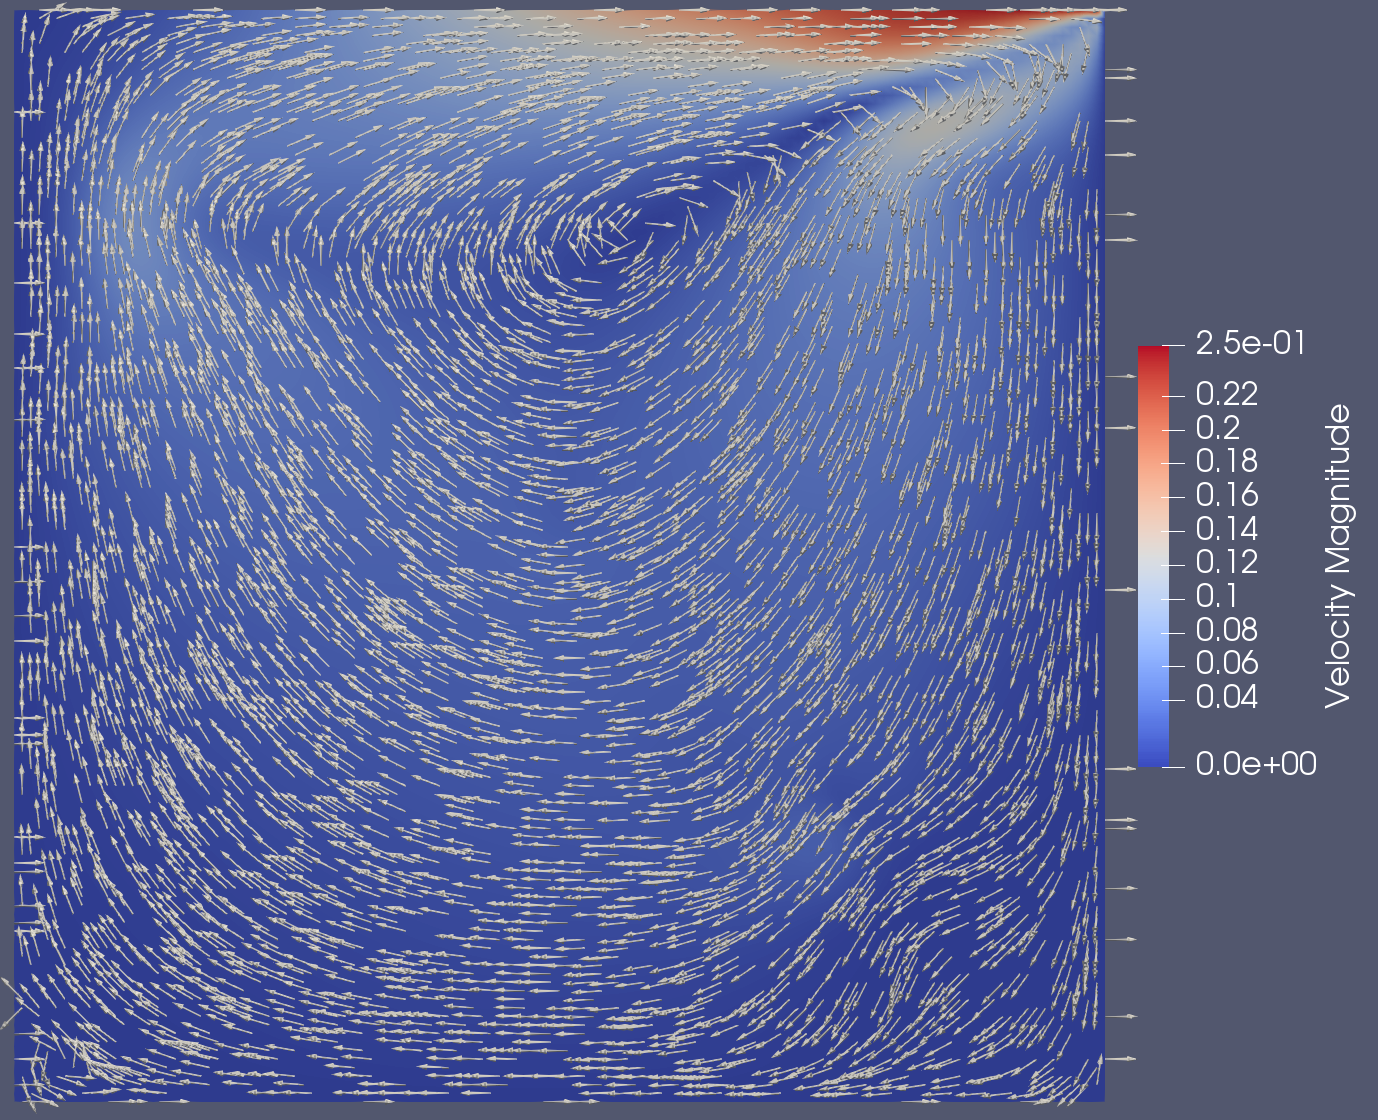
\includegraphics[width=\textwidth]{stokes-velocity}
      \end{column}
      \begin{column}{0.333\pagewidth}
        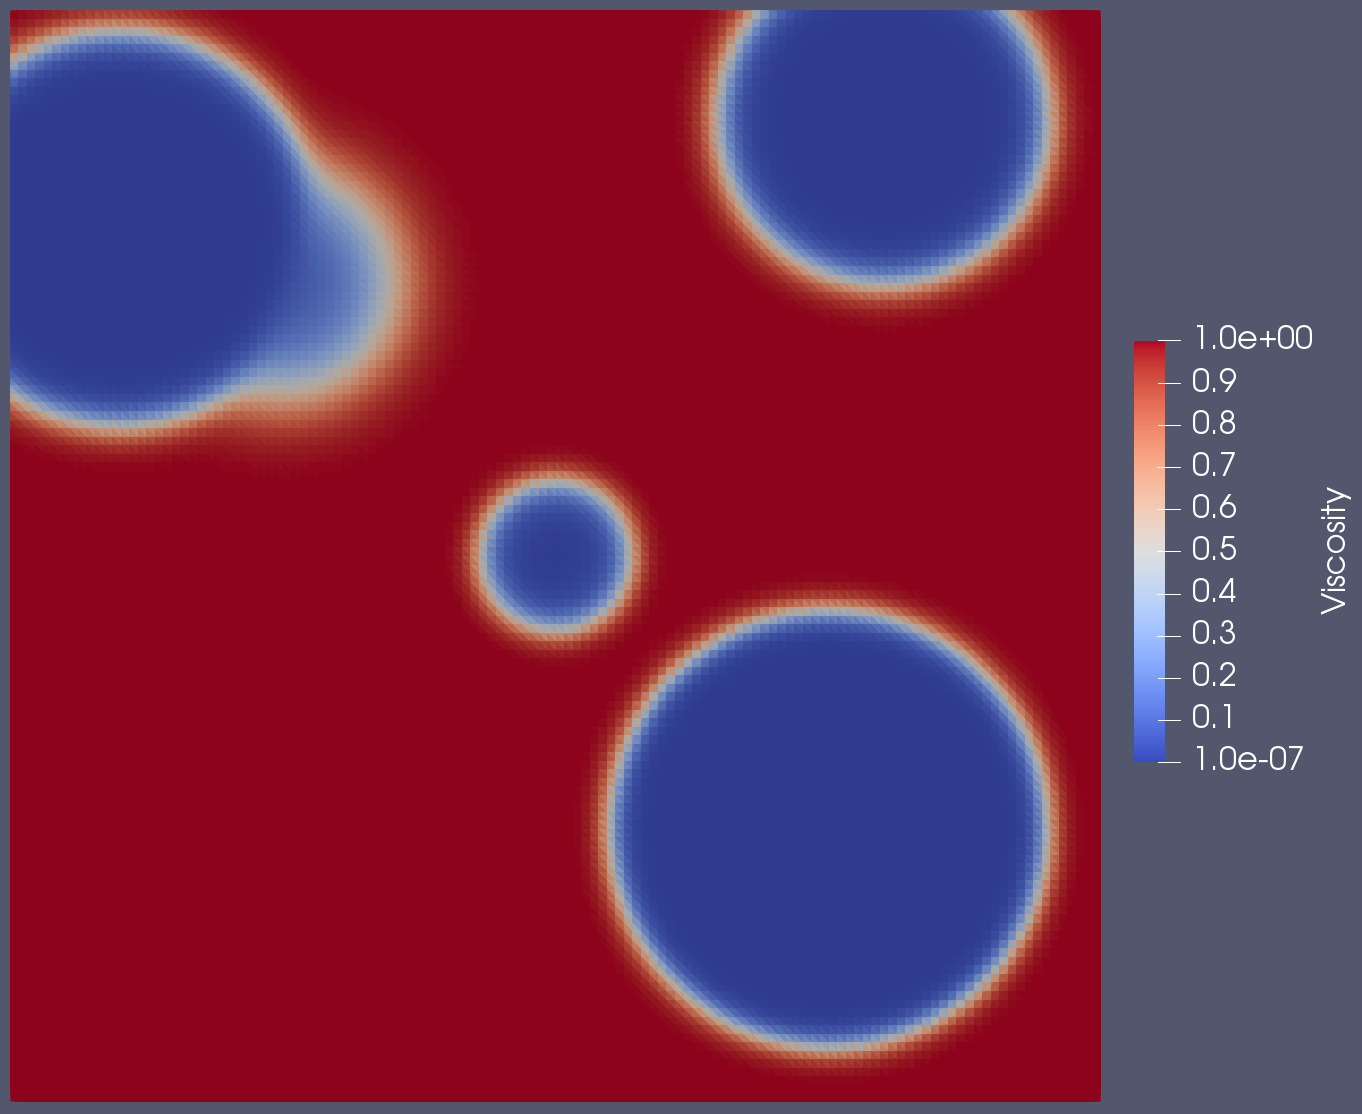
\includegraphics[width=\textwidth]{stokes-viscosity}
      \end{column}
      \begin{column}{0.333\pagewidth}
        \begin{itemize}
        \item Converges in around 16 iterations, even with large
          viscosity contrasts (Gaussian bumps)
        \item Falls over when jumps appear
        \end{itemize}
      \end{column}
    \end{columns}
  \end{onlyenv}
\end{frame}

\begin{frame}
  \frametitle{Hot off the press}

  TODO: Some N-S with S-V results here?
\end{frame}

\begin{frame}
  \frametitle{Conclusions}
  \begin{itemize}
  \item Bidirectional solver/discretisation interface useful
  \item Playground for preconditioner design: it's easy to get all the
    operators you need
  \item With scalability to large problems
  \item Overlapping Schwarz methods also benefit from this
  \item With topological decompositions in hand, can provide a
    \emph{generic} interface, encompassing many useful smoothing schemes
  \end{itemize}

  \pause

  \begin{center}
    Thanks!
  \end{center}
\end{frame}

\appendix
\begin{frame}[allowframebreaks]
  \frametitle{References}
  \printbibliography[heading=none]
\end{frame}


\end{document}

